\appendix

%%%%%%%%%%%%%%%%%%%%%%%%%%%%%%%%%%%%%%%%%%%%%%%%%%%%%%%%%%%%%%%%%%%%%%%%
\section{Performance evaluation} \label{appendix:perf-eval}
%%%%%%%%%%%%%%%%%%%%%%%%%%%%%%%%%%%%%%%%%%%%%%%%%%%%%%%%%%%%%%%%%%%%%%%%

In this section we report additional performance measurements for \sys.
%to gauge how well it meets its goals.

\textbf{Methodology.} We recorded timestamps while our code is
executing using the Performance Web API\footnote{Note that while this
  API normally reports values as doubles, due to recent security
  threats, such as Spectre~\cite{DBLP:journals/corr/abs-1801-01203},
  several browser developers have implemented countermeasures by
  reducing the precision of the DOMHighResTimeStamp
  resolution~\cite{reducetimeprecision,resolutionconsiderations}. In
  particular, Firefox reports these values as integer
  milliseconds. For our tests, we re-enabled higher precision values.}

While our extension's functionality only applies at the network level,
there is potential slowdown at the DOM processing level due to the
optimization techniques the browser applies throughout several levels
of the web page load pipeline. \autoref{fig:navigationtiming} shows
the different timestamps provided by the Navigation Timing
API~\cite{navigationtiming}, as well as a high-level description of
the browser processing model. Since our filter listens on the
onBeforeRequest event, none of the previous steps before Request are
affected. In this section, we refer to the difference in time between
responseEnd and requestStart as the "network filter time".

\begin{figure}[h]
	\begin{center}
 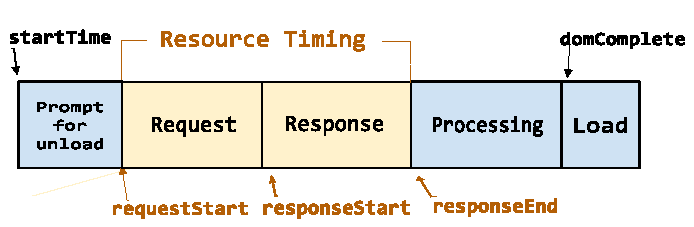
\includegraphics[scale=0.65]{img/timestamp-diagram-edited.pdf}
 \end{center}
 \caption{The Navigation Timing API's timestamps\protect\footnotemark}
 \label{fig:navigationtiming}
 \end{figure}

\footnotetext{This image was taken from the w3 spec: \url{https://www.w3.org/TR/navigation-timing-2/}}


\subsection{Top websites load times; continued} \label{top_sites}

\iffalse
\begin{figure}[h]
	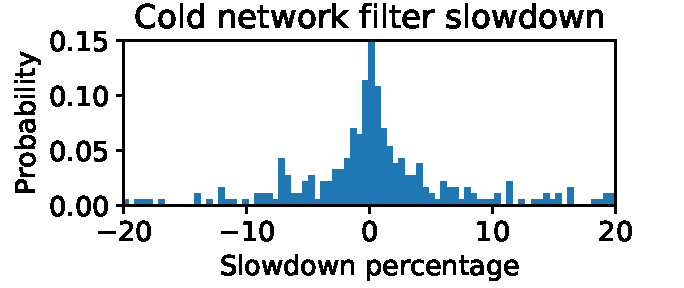
\includegraphics[scale=0.5]{results/density_histogram_filter_slowdown_small.pdf}
	\caption{Density histogram of network filter slowdown for top sites.}
	\label{fig:histogram_slowdown}
\end{figure}


Figure ~\ref{fig:histogram_slowdown} shows a closer look at the distribution for the cold network filter slowdown on the top sites (same values as in \autoref{fig:overall_slowdown}). For this component, 87.6\% of the slowdown values are less than 10\%.
\fi

\begin{figure}[h]
	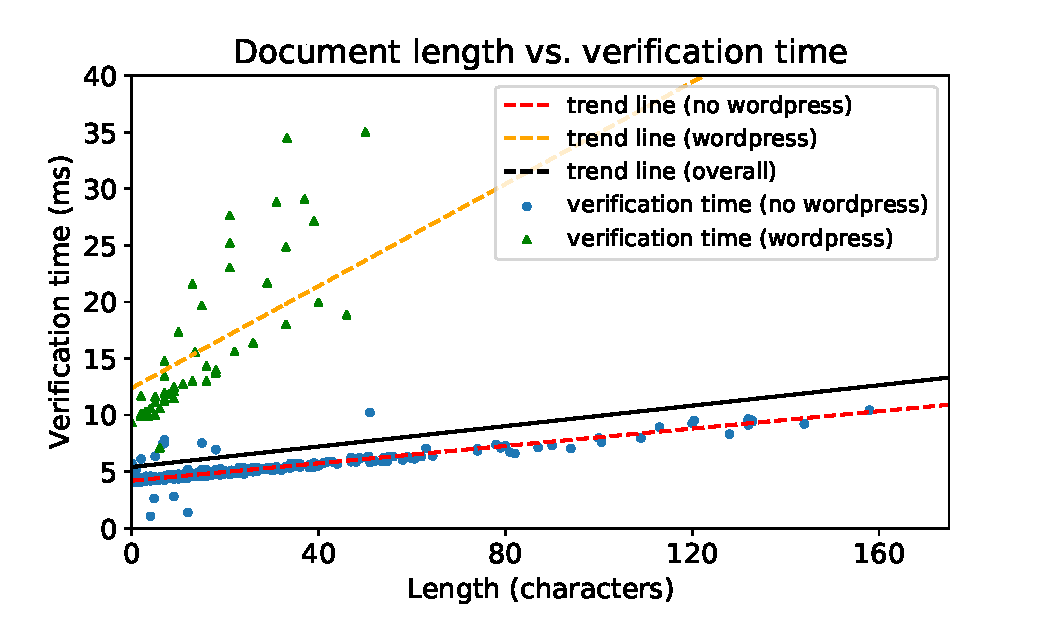
\includegraphics[scale=0.5]{results/string_length_vs_verification_time_small.pdf}
	\caption{Scatter plot of network filter time as a function of character length for top sites.}
	\label{fig:verification_time_string_length}
\end{figure}

 \autoref{fig:verification_time_string_length} shows the time spent by the call to our string verification function in the network filter as a function of the length of the string to be verified, differentiating between websites for which some probes tested positive and ones which no probes did. We applied least squares regression to calculate the shown trend lines. The Spearman's rank \footnote{The Spearman's correlation coefficient measures the strength and direction of association between two ranked variables: https://statistics.laerd.com/statistical-guides/spearmans-rank-order-correlation-statistical-guide.php} correlation values for no probe, probe, and overall are 0.91, 0.91, and 0.72 respectively, demonstrating positive correlation. Since both our probes and signatures use regex matching, we expect both trend lines to be linear, as seen in the graph. We expect the slope of the line to be higher when a probe passes, as it performs additional string verification. Around 37.4\% of all web sites use frameworks covered by our probes~\cite{w3stats}, thus, we expect the impact of our network filter to be closer to the non-probe values, as corroborated by our overall trend line.

\subsection{WordPress websites load times} \label{wordpress_sites}

We ran similar experiments as in ~\autoref{performance} and ~\autoref{top_sites}, but with the WordPress sites described in ~\autoref{methodology}. Thus, all of these have either one or multiple injection points in their HTML, and the network filter will spend an additional amount of time sanitizing these as defined by the signatures.

We report a slowdown of less than 10\% for 60\% of sites, and less than 40\% for 96.25\% of them. In the case of 'warm network filter', we report a higher slowdown, with less than 40\% for 60\% of sites. We believe this to be the case because the locally hosted pages decrease the network component time, causing any overhead to be seen as relatively high. However, as 48\% of the original values were below 60ms, we conclude a small impact on user experience as well.

%\begin{figure}[h]
%	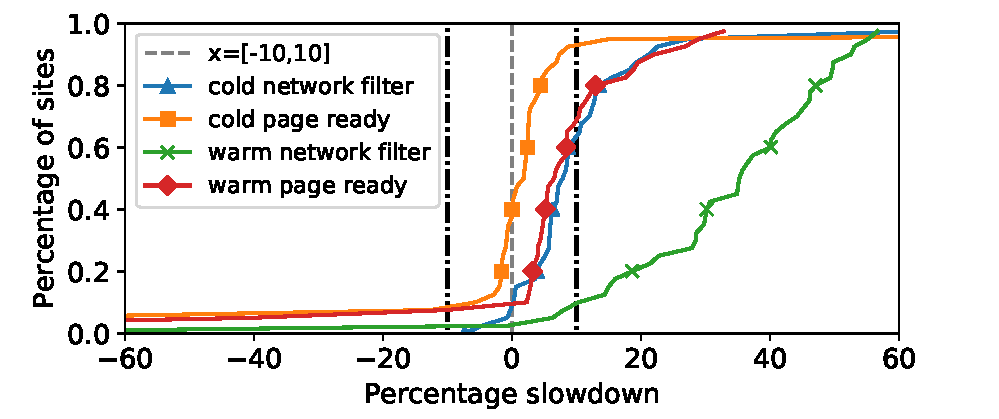
\includegraphics[scale=0.5]{results/extension_slowdown_wordpress_small.pdf}
%	\caption{Cumulative distribution of relative percentage slowdown with extension installed for WordPress sites.}
%	\label{fig:WordPress_slowdown}
%\end{figure}

\iffalse
\autoref{fig:histogram_slowdown_wordpress} shows the probability density of the cold network filter slowdown. In this case, we see that the distribution is skewed more towards a higher slowdown. As it is harder to discern the trend for this data set than its top site counterpart, we have also plotted the normal distribution of the data between 3 standard deviations. 65\% of values are less than 10\%.

\begin{figure}[h]
	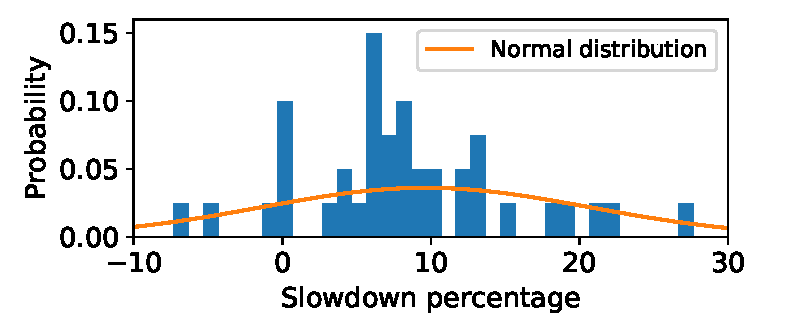
\includegraphics[scale=0.5]{results/density_histogram_filter_slowdown_wordpress_small.pdf}
	\caption{Density histogram of network filter slowdown for WordPress sites.}
	\label{fig:histogram_slowdown_wordpress}
\end{figure}
\fi

Finally, for string verification time as a function of document length for the WordPress sites, we report a linear trend with  Spearman's rank correlation of 0.630. In this case, all times were below 20 ms, with 90\% below 10 ms.


%\begin{figure}[h]
%	\begin{center}
%	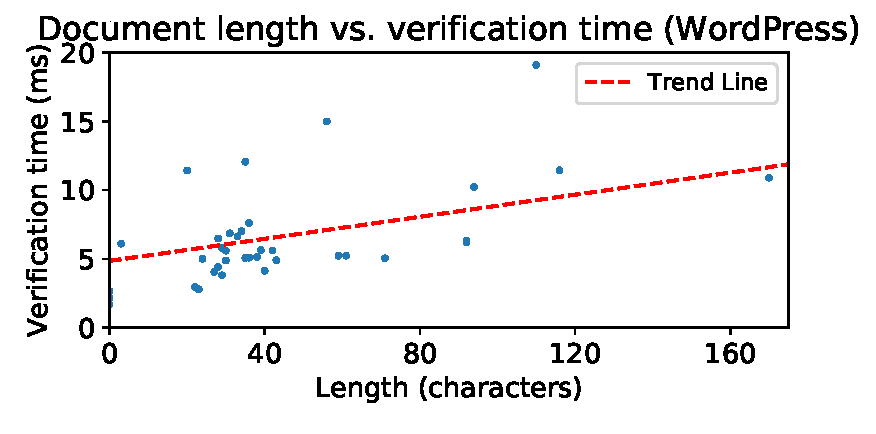
\includegraphics[scale=0.55]{results/string_length_vs_verification_time_wordpress_small.pdf}
%	
%	\caption{Scatter plot of network filter time as a function of character length for WordPress sites.}
%	\label{fig:verification_time_string_length_wordpress}
%\end{center}
%\end{figure}




%%%%%%%%%%%%%%%%%%%%%%%%%%%%%%%%%%%%%%%%%%%%%%%%%%%%%%%%%%%%%%%%%%%%%%%%
\subsection{Signature Language Description} \label{appendix:language_specification}
%%%%%%%%%%%%%%%%%%%%%%%%%%%%%%%%%%%%%%%%%%%%%%%%%%%%%%%%%%%%%%%%%%%%%%%%

We provide further description of our signature language:
\begin{itemize}
	\item
	url: If the exploit occurs in a specific URL or subdomain, this is defined as a string, e.g.
	\url{/wp-admin/options-general.php?page=relevanssi\%2Frelevanssi.php}, otherwise null.
	\item
	software: The software framework the page is running, e.g. WordPress. Some pages
	might not have a framework.
	\item
	softwareDetails: If running any software, this provides further information about when to load a signature. For WordPress, these are plugin names.
	\item
	version: The version number of the software/plugin/page, used for versioning as described in \autoref{filtering_process}.
	\item 
	type: Parameter for describing the signature type, 'string' describes a basic signature, 'listener' describes a signature with a listener for additional network requests.
	\item 
	sanitizer: The sanitizer to be used, "DOMPurify", "escape", or "regex". The default is DOMPurify.
	\item
	config: Additional config parameters to go along with the chosen sanitizer. For example, DOMPurify allows config through its API (i.e, DOMPurify.sanitize(dirty, config).
	\item
	typeDet: A string describing the recurrence of injection points throughout the document, e.g. 'single-unique', as described in ~\autoref{multiple_injections}.
	\item
	endPoints: An array of startpoint and endpoint tuples, specified as strings for regex matching.
	\item 
	endPointsPositions: An array of integer tuples, these are useful when one of the endPoints appears a multiple but fixed amount of times in the document, but only a few of them are injection points.
\end{itemize}

Additionally, if the value of type is `listener', the signature will have an additional field called listenerData, similar to a regular signature, describing the type of request to listen for.
